Ahora observemos las componentes de nuestra serie de tiempo. Cabe mencionar que las características de nuestra serie nos darán como resultado componentes diferentes a las que se acostumbró ver en la modelación ARIMA.
\\\\
Utilizando la función decompose como si se tratara de un modelo aditivo podremos acceder rápidamente a las componentes. A continuación podemos ver nuestra componente de tendencia, que tal y como se esperaba, no se alejó mucho del cero.

\begin{figure}[!ht]
    \centering
    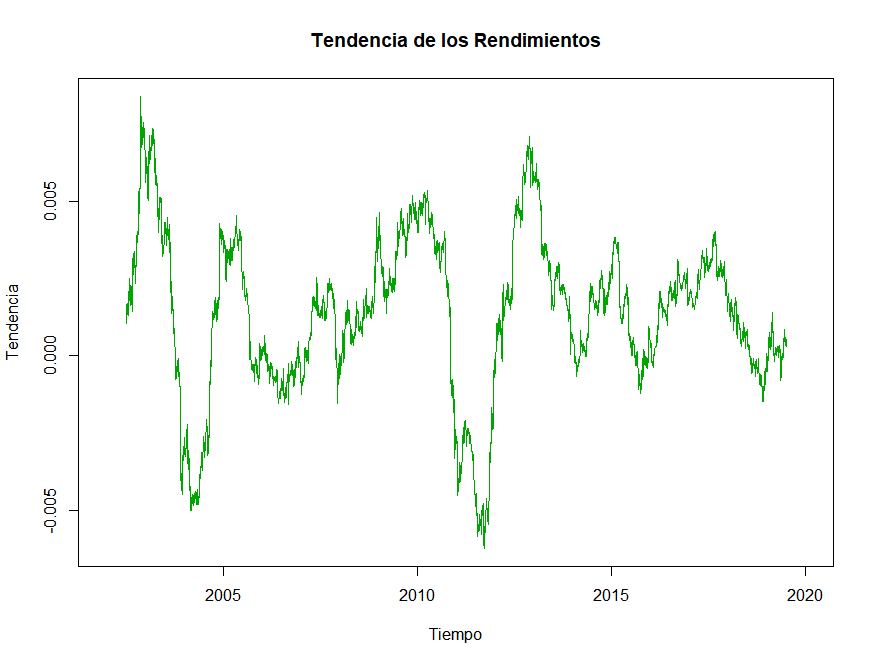
\includegraphics[scale=.35]{Graficos/CompRendimientos.png}
    \caption{Componente de tendencia de los rendimientos}
    \label{comp_tendencia}
\end{figure}

\newpage
La siguiente gráfica a observar será la de nuestra componente de ciclos estacionales. Podemos notar ligeramente que se tratan de ciclos anuales lo cual tiene sentido, al tratarse de rendimientos de acciones a pesar de su alta volatilidad, hay épocas que destacan por la reactivación de la actividad económica a lo largo del año.

\begin{figure}[!ht]
    \centering
    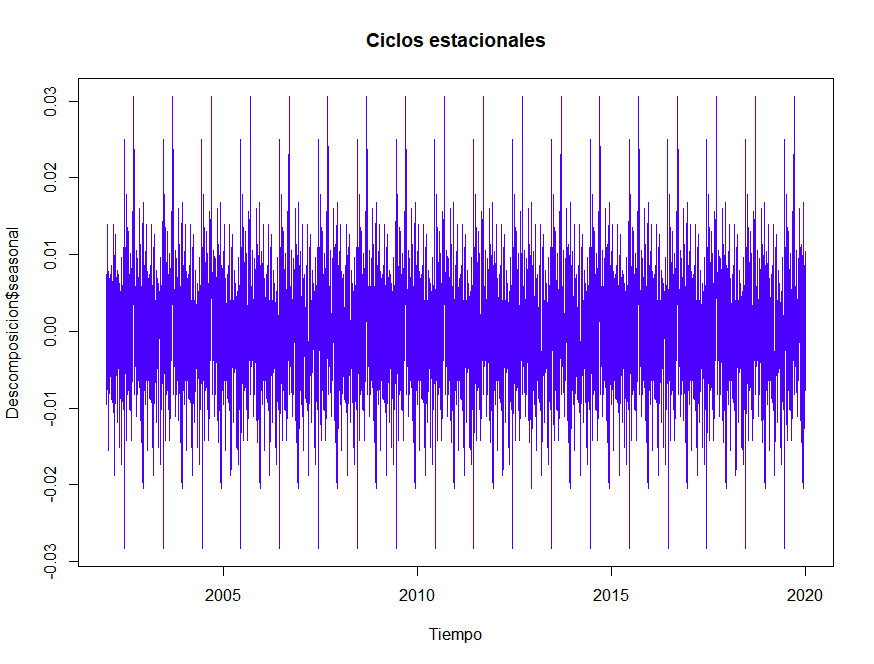
\includegraphics[scale=.35]{Graficos/CompCiclos.png}
    \caption{Componente de tendencia de los ciclos estacionales}
    \label{componente_ciclos}
\end{figure}


Finalmente observemos nuestra componente aleatoria. Trataremos de modelarla tomando en cuenta sus características de alta volatilidad.

\begin{figure}[!ht]
    \centering
    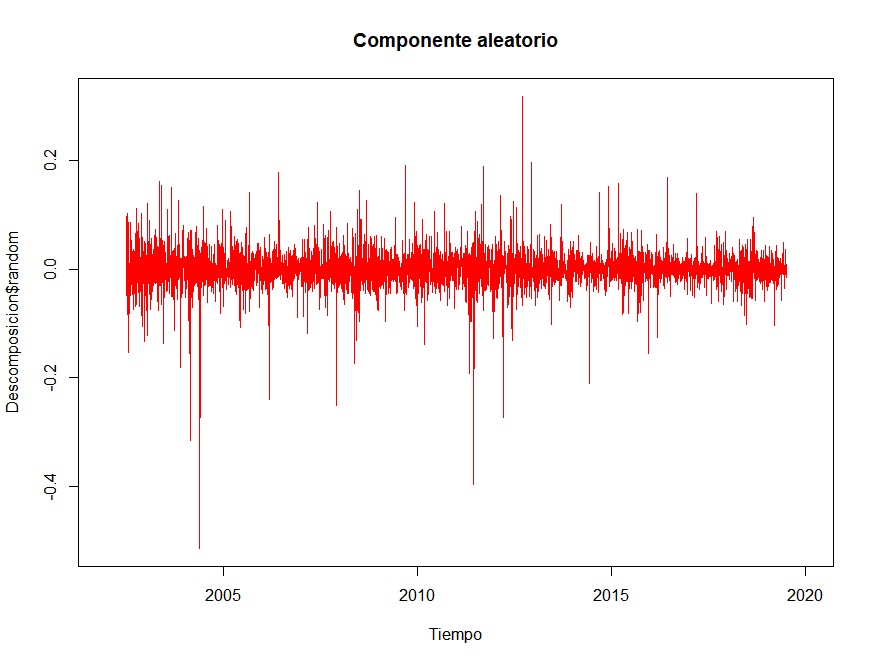
\includegraphics[scale=.33]{Graficos/CompRand.png}
    \caption{Componente aleatoria de los rendimientos}
    \label{componente_aleatoria}
\end{figure}

\newpage